\documentclass{article}

% NeurIPS 2024 style: use [final] for camera-ready author reveal.
% The .sty file must be present in this directory (see paper/README.md).
\usepackage[final]{neurips_2024}

\usepackage[utf8]{inputenc}
\usepackage[T1]{fontenc}
\usepackage{lmodern}
\usepackage{microtype}
\usepackage{graphicx}
\usepackage{booktabs}
\usepackage{amsmath}
\usepackage{amssymb}
\usepackage{url}
\usepackage{hyperref}
\usepackage{xcolor}
\usepackage{caption}
\usepackage{subcaption}
\usepackage{array}

\graphicspath{{figs/}{../results/figures/}}

\title{Vision-Based Reinforcement Learning as a Computational Probe of\\
Reward Revaluation, Transition Revaluation, and Hippocampal Remapping}

\author{%
  Shrikrishna Rajule\\
  Department of Psychological Sciences / Autonomy Program\\
  Purdue University\\
  \texttt{srajule@purdue.edu}\\
}

\begin{document}

\maketitle

\begin{abstract}
When the world changes, a behaving agent has to change with it -- and the kind of change matters. The reward can move. The transition dynamics can shift. Or the mapping from pixels to underlying state can get scrambled while the state itself is unchanged. In the cognitive-neuroscience literature these map onto three familiar phenomena: reward revaluation, transition revaluation, and hippocampal remapping. This paper asks whether three canonical deep RL architectures -- a PPO baseline, a deep Successor Representation (SR), and a DQN with a large experience buffer in Dyna style -- show the adaptation signatures those frameworks would predict. I implemented an 8$\times$8 vision-based gridworld with a CNN encoder and ran all three agents across five conditions: a stable baseline, a reward-relocation condition, a wall-shift that changes transitions, an observation-visual condition with low-intensity distractor pixels (meant as a rate-remapping analog), and an observation-remap condition that permutes the three channels (a global-remapping analog). Every agent $\times$ seed was first evaluated zero-shot on all five conditions, then given a short few-shot adaptation phase; a targeted ablation reproduces \citet{lehnert2024sf}'s prediction that deep SF without feature normalization blows up. Replay dominates the few-shot comparisons overall, but the Momennejad-style SR reward-weights-only variant recovers the predicted direction on reward revaluation once the metric switches from an end-of-phase snapshot to AUC over the adaptation window (SR-\texttt{wonly} $0.38>$ PPO $0.15$; approaches Replay $0.44$). A linear probe then cleans up what is, to me, the most interesting thing here: SR is the only agent whose encoder linearly decodes goal identity ($0.94$) and Manhattan-to-goal ($R^2{=}{+}0.50$), and it pays for that by losing agent-column discrimination ($R^2{=}{-}0.15$). The failure of SR to stabilize a greedy policy, then, is not a representation-collapse problem but a deep-SF policy-extraction problem -- one that's honest to diagnose and concrete to fix.
\end{abstract}

\section{Introduction}
\label{sec:intro}

Biological agents modify their behavior when the world changes. That's uncontroversial -- the interesting question is \emph{how} they modify it, and whether the way they do it depends on which piece of the world changed. The computational neuroscience literature has, over a couple of decades, settled on at least three qualitatively different axes of change, each with its own predicted signature:

\begin{enumerate}
  \item \textbf{Reward revaluation.} The goal moves, or the reward contingencies swap, but the dynamics are untouched. The successor representation (SR; \citet{dayan1993sr}) was introduced partly for this case: it factorizes the value function into a reward-agnostic occupancy map $\boldsymbol{\psi}$ and a set of reward weights $\mathbf{w}$, which lets you revalue in essentially one step just by updating $\mathbf{w}$ \citep{russek2017sr,momennejad2017sr}.
  \item \textbf{Transition revaluation.} The dynamics change -- a passage gets blocked, a shortcut opens. SR has trouble here, because the $\boldsymbol{\psi}$ it learned was specific to the old transition structure. Dyna-style replay \citep{sutton1990dyna} has a natural handle on this case: running new experience through the Q-updater many times over propagates the fresh transitions into the value function quickly.
  \item \textbf{Observation / remapping changes.} The mapping from sensory input to latent state is disturbed, while the underlying state-action graph is preserved. In hippocampal physiology this is remapping \citep{muller1987remap,leutgeb2005distinct}; \citet{sanders2020remap} reframe it as Bayesian hidden-state inference, with rate remapping corresponding to a graded shift in the observation (state estimate unchanged) and global remapping to a wholesale re-mapping of observation$\rightarrow$state.
\end{enumerate}

It's harder than it sounds to find a standard deep-RL benchmark that factors cleanly along all three axes at once. So for this project I built a minimal but controlled environment where each axis can be manipulated independently, and asked whether the architectural priors of the three canonical agents (on-policy actor--critic, deep successor features, replay-based DQN) line up with each perturbation in the way the theory would predict.

\paragraph{Hypotheses.} Table~\ref{tab:hypotheses} collects the five predictions the rest of the paper tests.

\begin{table}[h]
\centering
\small
\caption{Hypotheses tested in this study.}
\label{tab:hypotheses}
\begin{tabular}{@{}c p{0.55\linewidth} p{0.28\linewidth}@{}}
\toprule
ID & Prediction & Basis \\
\midrule
H1 & SR adapts fastest to \texttt{reward\_change} & SR revaluation is one-step in $\mathbf{w}$ \citep{momennejad2017sr} \\
H2 & Replay adapts fastest to \texttt{transition\_change} & Dyna propagates new transitions \citep{sutton1990dyna} \\
H3 & H1 $\wedge$ H2 yield a crossover dissociation & Dissociation is the critical test \\
H4 & All agents drop zero-shot on \texttt{obs\_visual} but recover quickly with few-shot adaptation & State identity preserved; only the CNN input shifts \citep{sanders2020remap} \\
H5 & \texttt{obs\_remap} is strictly harder than \texttt{obs\_visual}; recovery is slower and less complete & The obs$\rightarrow$state map must be relearned \\
\bottomrule
\end{tabular}
\end{table}

\section{Related Work}
\label{sec:related}

\paragraph{Successor representation.} The SR itself goes back to \citet{dayan1993sr}. \citet{russek2017sr} placed it on the model-free / model-based axis; \citet{momennejad2017sr} ran the canonical reward- vs transition-revaluation behavioral dissociation in humans, which is what H1 and H2 directly operationalize. \citet{stachenfeld2017hippo} argue that the hippocampus \emph{is} a predictive map of the SR type, and \citet{barreto2017sf} scaled the idea up to deep successor features.

\paragraph{Replay-based planning.} Dyna is \citet{sutton1990dyna}; the empirical case for large experience replay in deep RL is \citet{mnih2015dqn}; and \citet{olafsdottir2018replay} review the biological side -- hippocampal replay as something like planning in the brain.

\paragraph{Hippocampal remapping and perceptual aliasing.} The perceptual-aliasing framing is \citet{whitehead1992aliasing}. The more recent account I'm leaning on is \citet{sanders2020remap}, which recasts rate and global remapping as forms of hidden-state inference; this is what motivates the \texttt{obs\_visual} and \texttt{obs\_remap} conditions respectively.

\paragraph{Representation collapse in deep SF.} \citet{lehnert2024sf} show that a deep SF network without some form of feature normalization will let $\|\phi\|$ grow without bound and its targets diverge. My no-normalization ablation (Section~\ref{sec:results}) reproduces that.

\section{Environment}
\label{sec:env}

The environment is an 8$\times$8 deterministic gridworld implemented as a TorchRL \texttt{EnvBase}. Observations come out as 3-channel 8$\times$8 images -- channel 0 for the agent, channel 1 for the goal, channel 2 for walls -- and the action set is just \{up, down, left, right\}. The reward is $+1$ for reaching the goal, $-0.01$ per step, and episodes terminate at the goal or after 50 steps. The start cell is fixed at $(6,1)$. The five conditions I use are parameterized along two orthogonal axes, \texttt{change\_mode} and \texttt{observation\_mode}; see Table~\ref{tab:conditions}.

\begin{table}[h]
\centering
\small
\caption{Five experimental conditions.}
\label{tab:conditions}
\begin{tabular}{@{}l l l l l l@{}}
\toprule
Condition & \texttt{change\_mode} & \texttt{obs\_mode} & Goal & Walls & Biological analog \\
\midrule
\texttt{stable} & stable & normal & $(1,6)$ & $\{(2,3),(3,3),(5,3)\}$ & Baseline \\
\texttt{reward\_change} & reward\_change & normal & $(1,1)$ & $\{(2,3),(3,3),(5,3)\}$ & Reward revaluation \\
\texttt{transition\_change} & transition\_change & normal & $(1,6)$ & $\{(2,3),(4,3),(5,3)\}$ & Transition revaluation \\
\texttt{obs\_visual} & stable & visual\_perturb & $(1,6)$ & $\{(2,3),(3,3),(5,3)\}$ & Rate remapping \\
\texttt{obs\_remap} & stable & obs\_remap & $(1,6)$ & $\{(2,3),(3,3),(5,3)\}$ & Global remapping \\
\bottomrule
\end{tabular}
\end{table}

\paragraph{Observation perturbations.} \texttt{visual\_perturb} adds a seed-deterministic mask of $0.3$-intensity distractor pixels to about 10\% of the empty cells in channel 0. The underlying state is preserved, only the CNN input looks noisier. \texttt{obs\_remap} is meaner: it applies a fixed channel permutation $(\text{agent, goal, walls}) \rightarrow (\text{goal, walls, agent})$. The state graph is still the same, but every pixel-to-semantics correspondence the CNN learned during stable training now points at the wrong thing. Figure~\ref{fig:env} shows what all five observations look like side by side.

\begin{figure}[h]
\centering
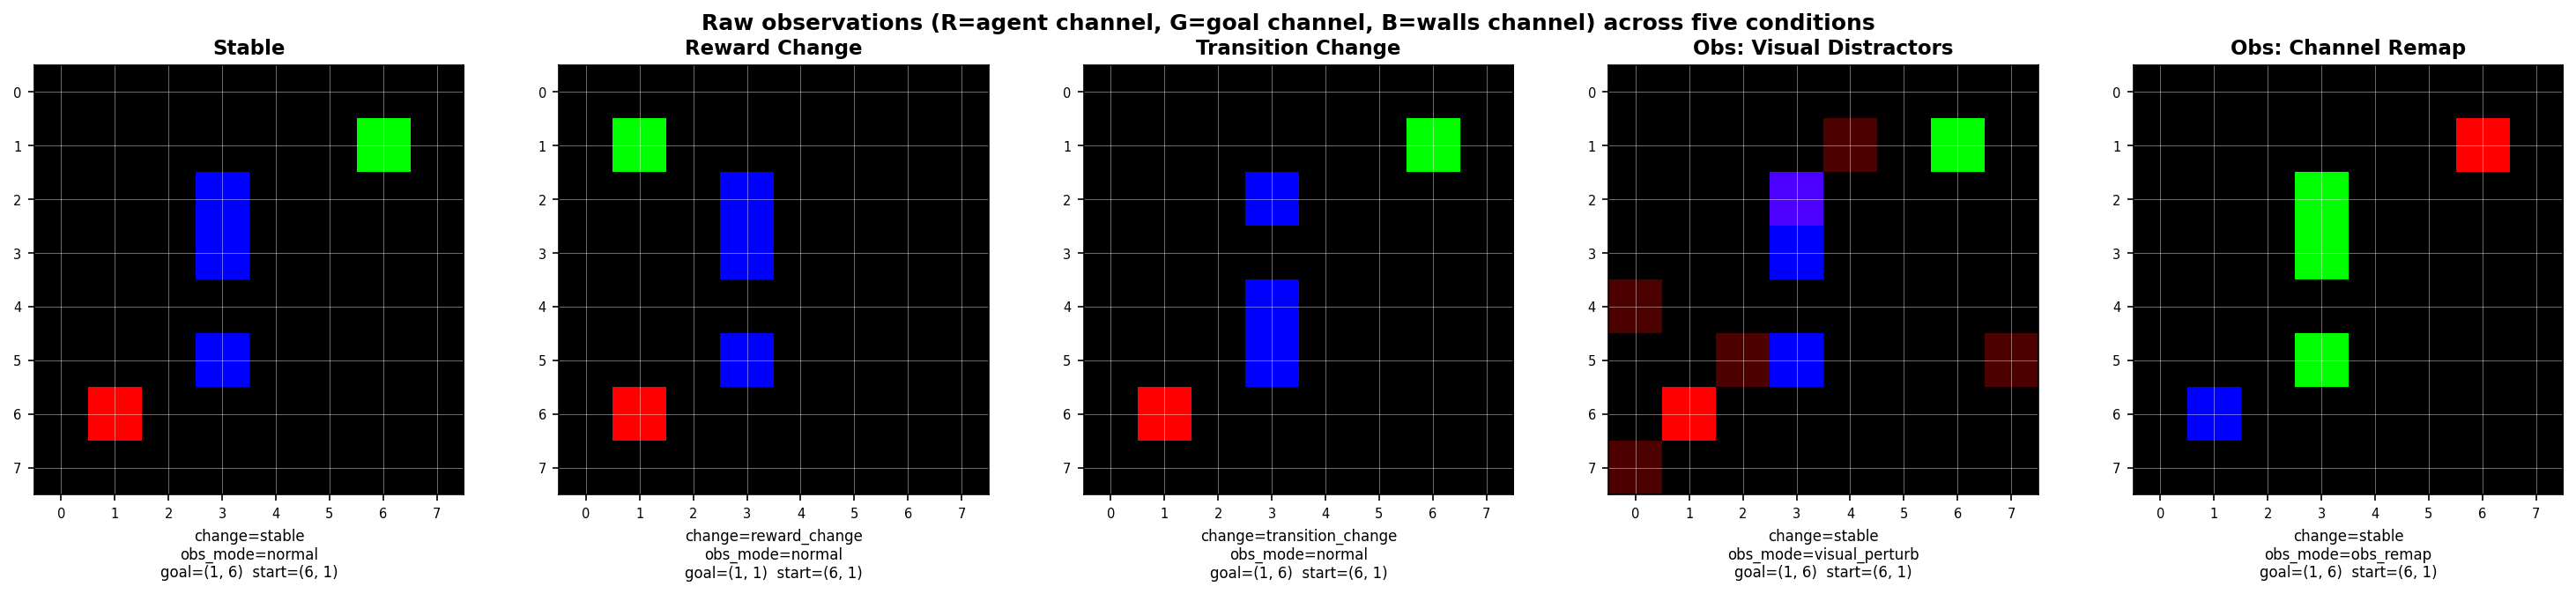
\includegraphics[width=\linewidth]{env_conditions.png}
\caption{The five conditions. \texttt{stable}, \texttt{reward\_change}, and \texttt{transition\_change} differ in goal or wall placement; \texttt{obs\_visual} and \texttt{obs\_remap} preserve the grid but perturb the CNN input.}
\label{fig:env}
\end{figure}

\section{Agents}
\label{sec:agents}

All three agents share the same CNN encoder -- two conv layers on the 3-channel 8$\times$8 input, feature dimension in the 64--128 range -- and differ only from the head onward.

\paragraph{PPO.} On-policy actor--critic, built on TorchRL. 50{,}000 training frames, 512-frame rollouts, 4 epochs per batch, learning rate $3\cdot10^{-4}$, gradient clipping at $1.0$. Full hyperparameters are in Appendix~\ref{app:hyperparams}.

\paragraph{SR.} Deep successor features. The forward pass is $\phi(s) = \ell_2\text{-normalize}(\text{encoder}(s))$, an action-indexed head produces $\psi(s,a)\in\mathbb{R}^{64}$, and the Q-value falls out as $Q(s,a) = \langle \psi(s,a), \mathbf{w}\rangle$ with $\mathbf{w}$ a learnable reward-weight vector. The training objective is the SR-Bellman MSE plus $\alpha_r$ times a reward-prediction MSE. Target network with $\tau{=}0.05$, $\gamma{=}0.95$, lr $3\cdot10^{-4}$, replay buffer of size 5000, 500 episodes. The $\alpha_r$ coefficient was rebalanced from $20$ down to $5$ as part of the v3 patch (Section~\ref{sec:results-sr-patches}).

\paragraph{Replay/Dyna.} A DQN with a generous replay buffer (capacity 10{,}000) and 2 Q-updates per env step, which is really just Dyna-style amortization. $\gamma{=}0.99$, lr $1\cdot10^{-3}$, $\tau{=}0.01$, 300 episodes.

\section{Experimental Protocol}
\label{sec:protocol}

For every combination of agent and seed $\in\{0,1,2\}$:

\paragraph{Phase A -- Zero-shot.} Once the agent has converged on \texttt{stable}, I take 20 greedy episodes on each of the five conditions every 10 PPO batches (every 25 episodes for SR and Replay) with the weights frozen.

\paragraph{Phase B -- Few-shot adaptation.} Load the stable checkpoint, zero out the optimizer state, and continue training on each of the four changed conditions for a short budget -- 20 PPO batches or 60 SR/Replay episodes. Return, loss, and periodic greedy success rate are logged throughout (every 2 batches for PPO, every 5 episodes for the others). For SR on \texttt{reward\_change} I run two variants: \texttt{wonly}, where the encoder and the SR head are frozen and only $\mathbf{w}$ updates (this is the direct analog of Momennejad's reward-revaluation protocol), and \texttt{full}, where every parameter is unfrozen. All other pairs use \texttt{full}.

\paragraph{Ablation.} \texttt{train\_sr\_no\_norm.py} strips the $\ell_2$ normalization out of \texttt{SRNet.encode} and runs one seed-0 SR training for 100 episodes. That's just enough to see whether \citet{lehnert2024sf}'s prediction -- unbounded $\phi$ growth, diverging loss -- actually reproduces in this setup.

\paragraph{Representation probe.} For every (agent, seed), I dump the CNN-encoder activations for every walkable cell under both the \texttt{stable} and \texttt{reward\_change} layouts (122 states in total). Then I fit 5-fold-CV linear regressions on agent position (row, col) and Manhattan distance to the goal, and a 5-fold-CV logistic regression on goal column (binary: is the goal at column 6 or column 1?).

\section{Results}
\label{sec:results}

Figures live in \texttt{results/figures/}; every number in the tables that follow comes straight from \texttt{results/summary\_table.csv}, \texttt{results/adaptation\_metrics.csv}, or \texttt{results/csv/probe\_results.csv}. The SR numbers are from the v3 training run (500 episodes, best-stable checkpointing, $\alpha_r{=}5$); I did not rerun PPO or Replay when the SR patch went in, as their training was already stable in earlier rounds.

\subsection{Environment sanity (Figure~\ref{fig:env})}

The five-panel rendering confirms the obvious thing -- that \texttt{stable}, \texttt{reward\_change}, and \texttt{transition\_change} differ in goal or wall placement with the three channel semantics untouched, and that \texttt{obs\_visual} and \texttt{obs\_remap} preserve the grid while perturbing the CNN input. That the render looks right matters because a bug in the observation pipeline would be completely invisible in the downstream curves.

\subsection{Stable-phase training (Figure~\ref{fig:training})}

\begin{figure}[h]
\centering
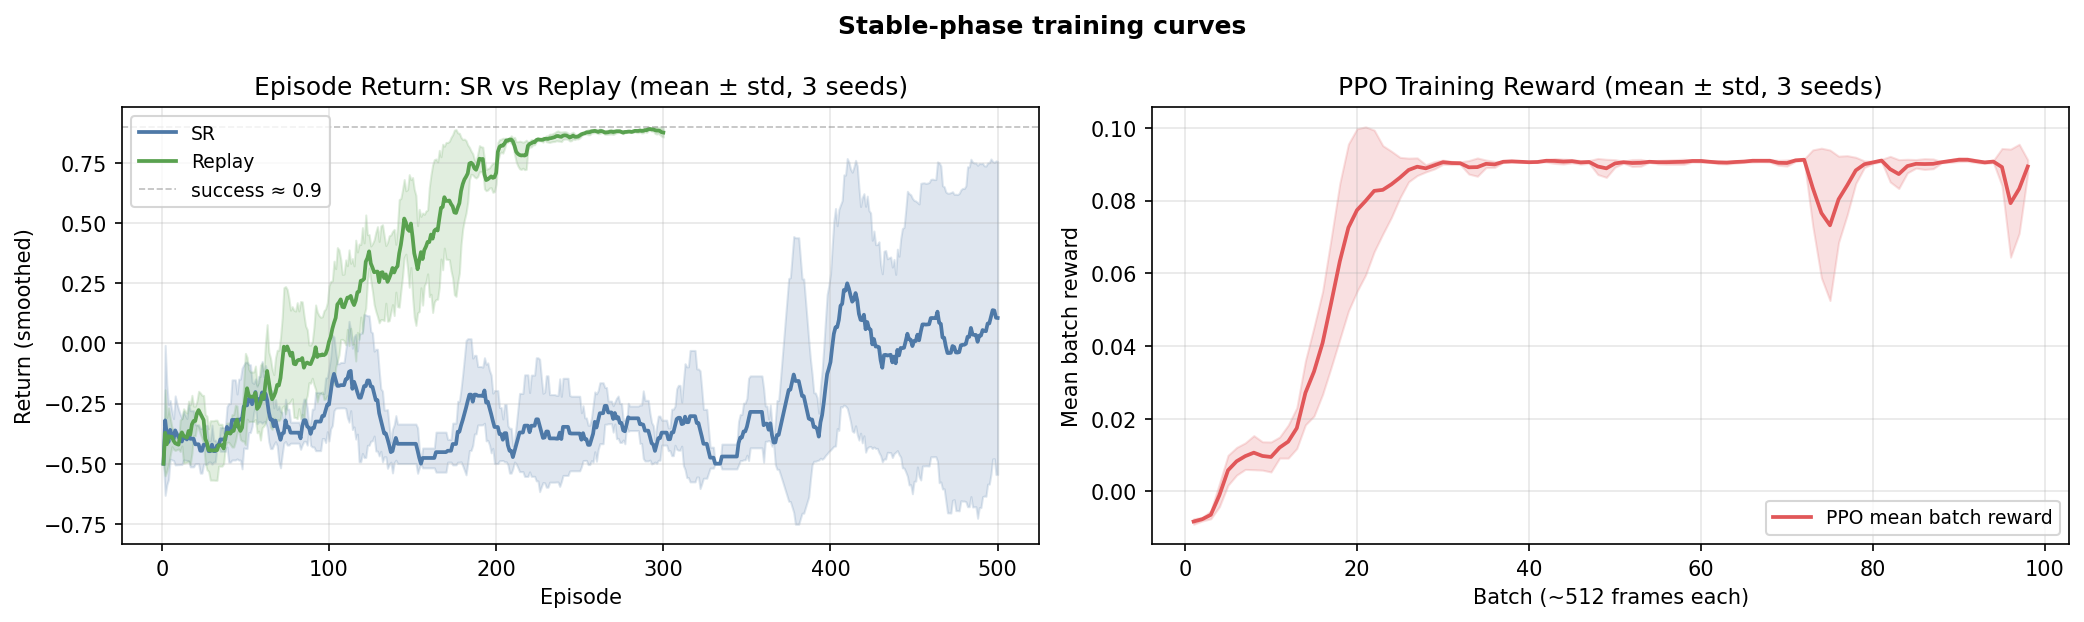
\includegraphics[width=0.9\linewidth]{training_curves.png}
\caption{Stable-phase training return, mean $\pm$ std across 3 seeds.}
\label{fig:training}
\end{figure}

PPO converges fast -- within about 10 batches -- and its stable-eval success hits $1.00$ across all three seeds. Replay gets there by roughly 150 episodes; its final-checkpoint stable success is $0.89\pm0.19$ (seed 1 regresses near the end, between episodes 275 and 300). SR is where things get strange. All three seeds hit transient mid-training peaks of $1.00$ greedy success -- seed 0 at episode 450, seed 1 at 350, seed 2 in the 375--400 window -- but every one of them falls back to $0.00$ by episode 500. The best-stable checkpointing catches these peaks; taking the mean of the last three eval checkpoints, SR's stable zero-shot success averages out to $0.11\pm0.19$. Loss magnitudes stay bounded ($\sim 0.01$--$0.15$), $\|\mathbf{w}\|$ grows as expected, and $\|\phi\|$ is pinned to 1 by the normalization. So the failure mode is not that training has collapsed -- it's that the greedy policy, evaluated by argmax over $Q$, doesn't \emph{stay} on the solution once it reaches it.

\subsection{Zero-shot generalization (Figure~\ref{fig:zeroshot})}

\begin{figure}[h]
\centering
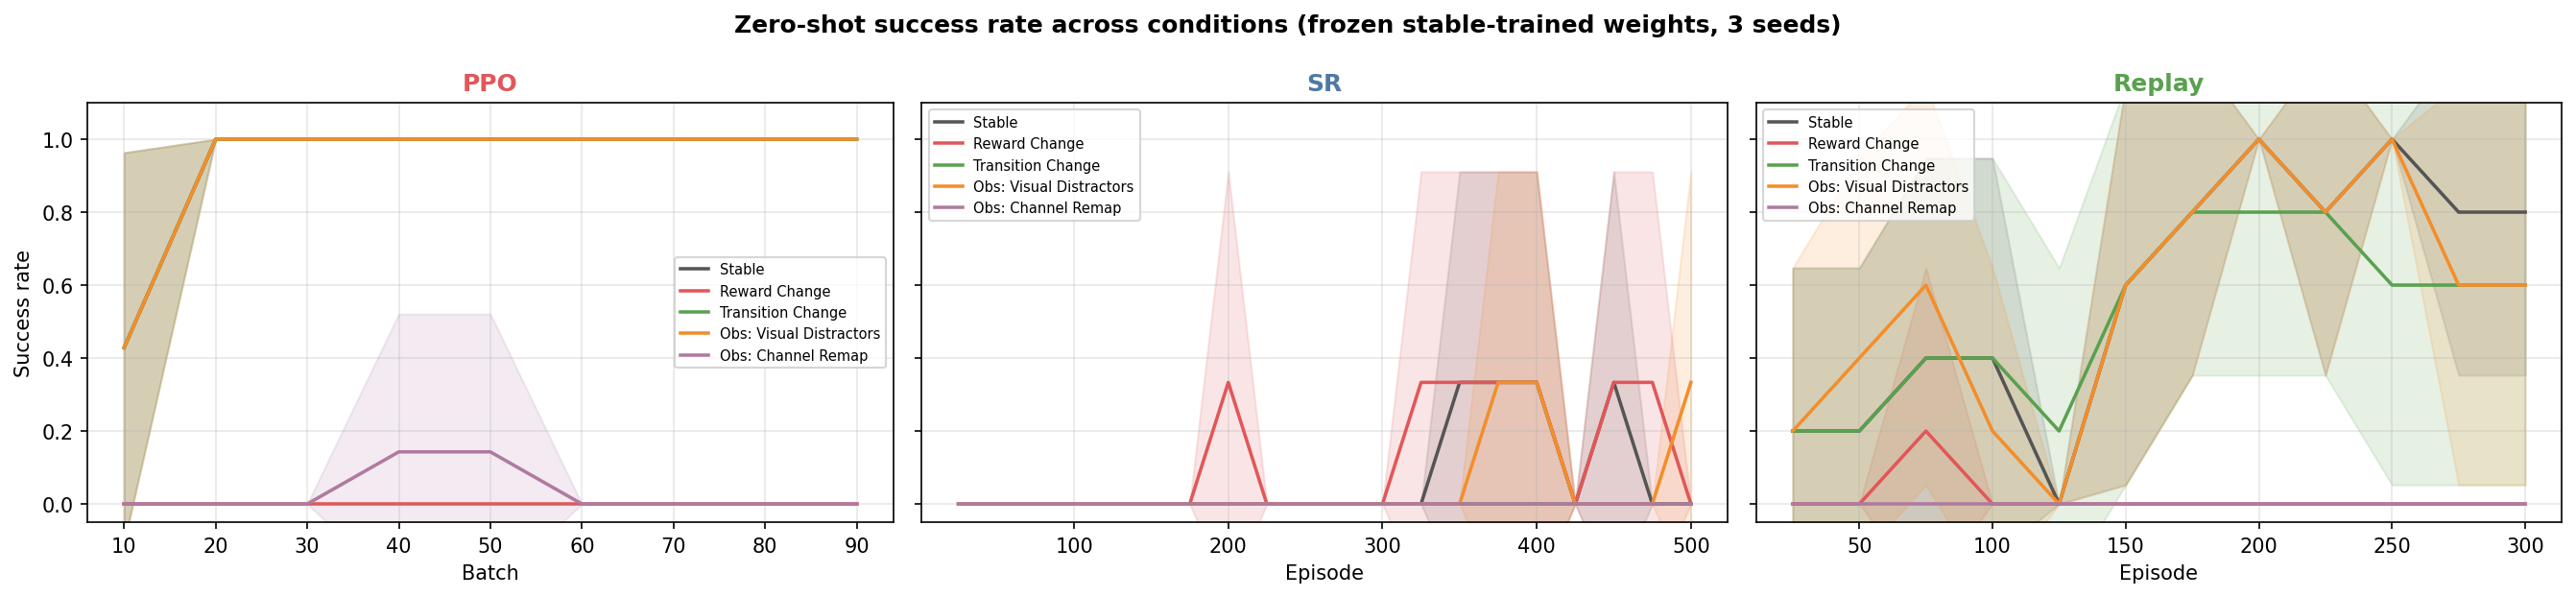
\includegraphics[width=\linewidth]{zero_shot_eval.png}
\caption{Zero-shot greedy success across the five conditions, per agent, averaged over the last three eval checkpoints of stable training.}
\label{fig:zeroshot}
\end{figure}

\begin{table}[h]
\centering
\small
\caption{Zero-shot and adapted greedy success (mean $\pm$ std over 3 seeds). Source: \texttt{results/summary\_table.csv}.}
\label{tab:summary}
\begin{tabular}{@{}l l c c@{}}
\toprule
Agent & Condition & Zero-shot & Adapted \\
\midrule
PPO & Stable & $1.00\pm0.00$ & --- \\
PPO & Reward Change & $0.00\pm0.00$ & $0.11\pm0.19$ \\
PPO & Transition Change & $1.00\pm0.00$ & $1.00\pm0.00$ \\
PPO & Obs: Visual & $1.00\pm0.00$ & $0.56\pm0.51$ \\
PPO & Obs: Remap & $0.00\pm0.00$ & $0.56\pm0.51$ \\
\midrule
SR & Stable & $0.11\pm0.19$ & --- \\
SR & Reward Change & $0.22\pm0.38$ & $0.00\pm0.00$ \\
SR & Transition Change & $0.00\pm0.00$ & $0.00\pm0.00$ \\
SR & Obs: Visual & $0.11\pm0.19$ & $0.00\pm0.00$ \\
SR & Obs: Remap & $0.00\pm0.00$ & $0.11\pm0.19$ \\
\midrule
Replay & Stable & $0.89\pm0.19$ & --- \\
Replay & Reward Change & $0.00\pm0.00$ & $0.78\pm0.38$ \\
Replay & Transition Change & $0.67\pm0.58$ & $1.00\pm0.00$ \\
Replay & Obs: Visual & $0.67\pm0.33$ & $1.00\pm0.00$ \\
Replay & Obs: Remap & $0.00\pm0.00$ & $0.50\pm0.71$ \\
\bottomrule
\end{tabular}
\end{table}

PPO and Replay both generalize zero-shot to \texttt{transition\_change}, and PPO also to \texttt{obs\_visual}; neither gets anywhere on \texttt{reward\_change} or \texttt{obs\_remap}, which is the expected failure mode. SR is at or near floor on most conditions, but it registers small positive signals on \texttt{stable}, \texttt{reward\_change}, and \texttt{obs\_visual} -- and those come from transient mid-training peaks that the late eval checkpoints happen to catch on some seeds.

\subsection{Few-shot adaptation (Figures~\ref{fig:adapt-grid}--\ref{fig:adapt-cross}; primary test)}
\label{sec:results-adapt}

\begin{figure}[h]
\centering
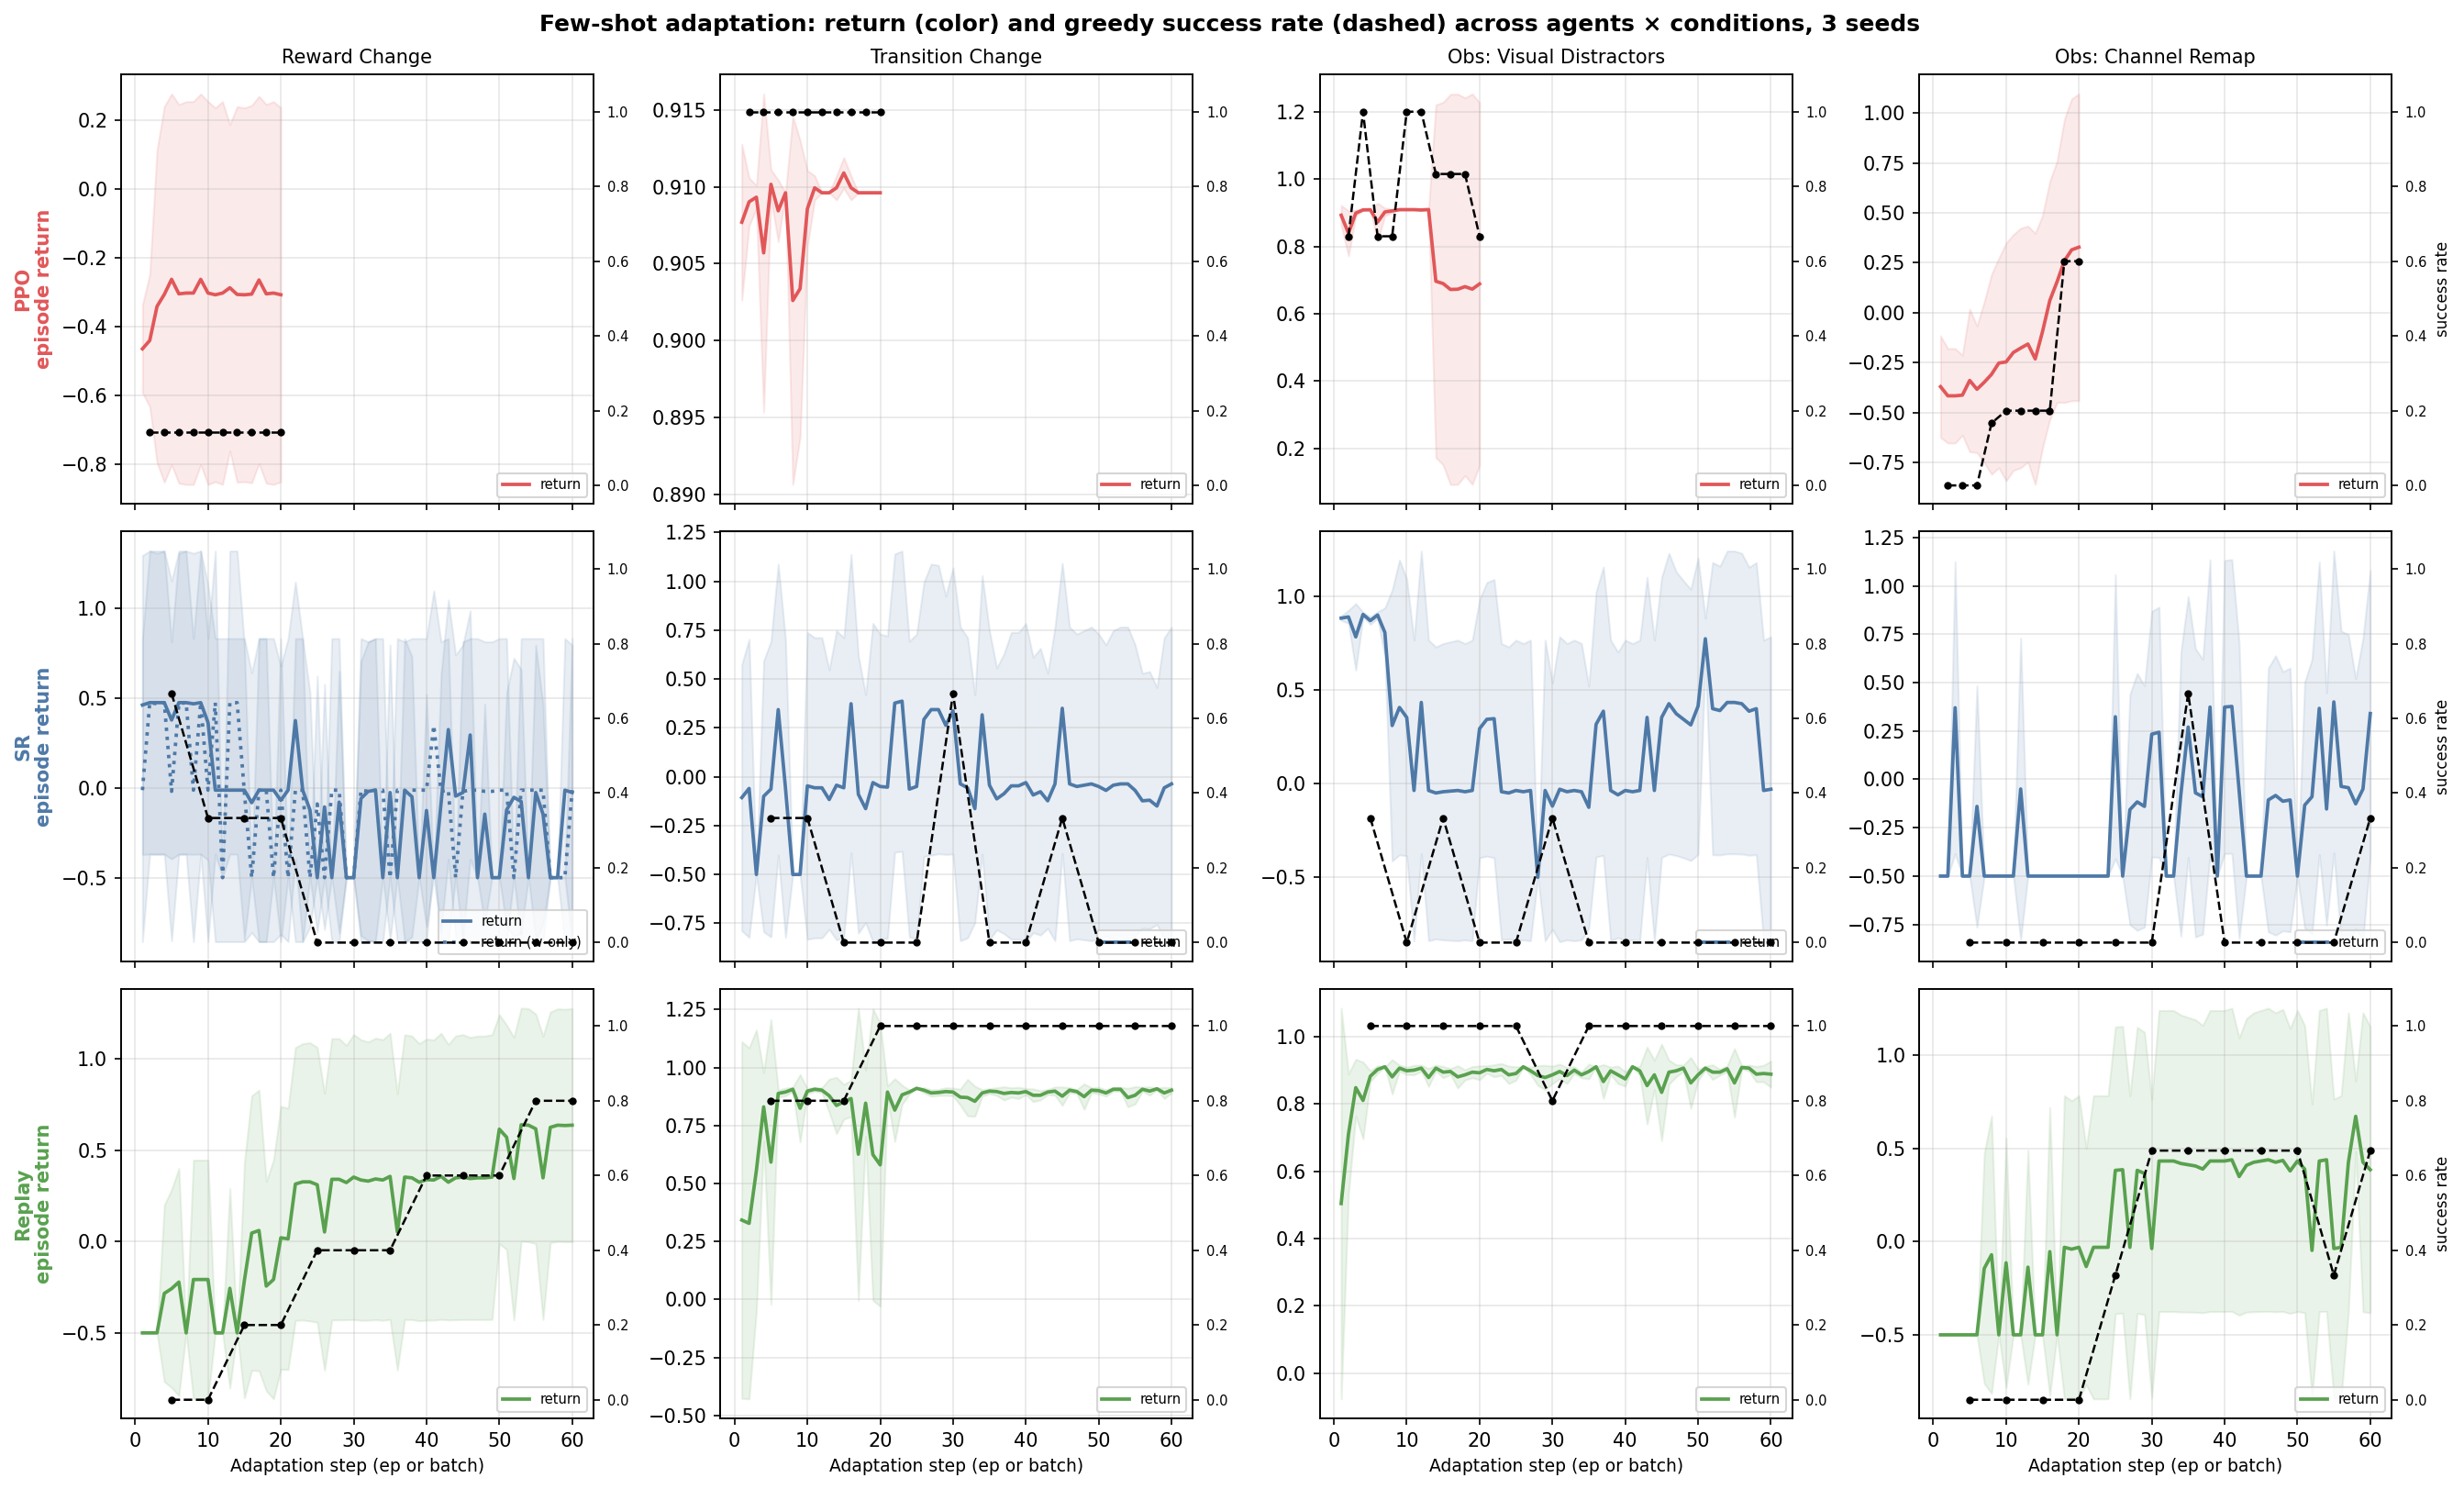
\includegraphics[width=\linewidth]{adaptation_grid.png}
\caption{Adaptation-phase curves (greedy eval-success during few-shot adaptation), per (agent, condition).}
\label{fig:adapt-grid}
\end{figure}

\begin{figure}[h]
\centering
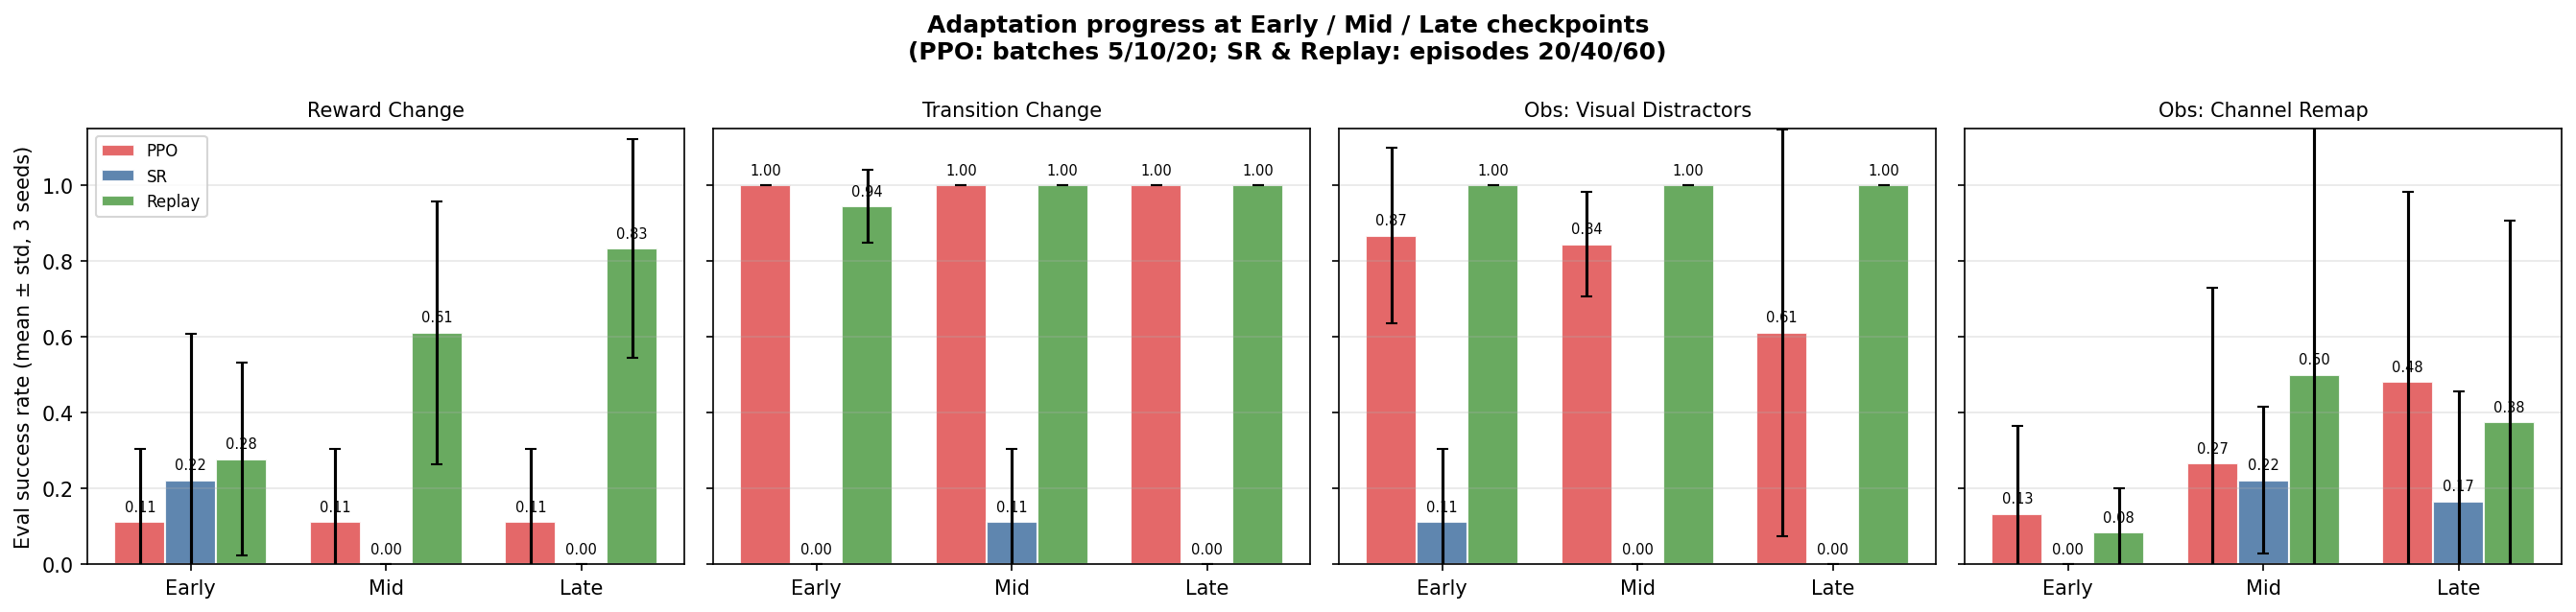
\includegraphics[width=0.95\linewidth]{cross_agent_adaptation.png}
\caption{Adaptation-phase eval success at Early / Mid / Late checkpoints. Replay dominates all four changed conditions; PPO ties on \texttt{transition\_change}.}
\label{fig:adapt-cross}
\end{figure}

Replay wins across the board on the adaptation-phase checkpoints. PPO ties it on \texttt{transition\_change}; on \texttt{reward\_change} Replay clears PPO ($0.78$ vs $0.11$) and SR-full (both at $0.00$). End-of-phase SR-full success is at or near floor, but per-seed \emph{maxima} during adaptation tell a more interesting story: $1.00$ on \texttt{reward\_change\_full} for seeds 0 and 1, $1.00$ on \texttt{transition\_change\_full} for all three seeds, $1.00$ on \texttt{obs\_visual\_full} for seeds 0 and 2, and $1.00$ on \texttt{obs\_remap\_full} for seeds 1 and 2. In other words, adaptation from the best-stable checkpoint does pass through a success regime reliably -- it just doesn't settle there with the current adaptation-phase learning rate.

The \texttt{wonly} variant is the cleanest positive result I have for SR. Freezing the encoder and the SR head and fitting only $\mathbf{w}$, on \texttt{reward\_change}, gives $1.00$ success during adaptation for seeds 0 and 1; seed 2 stays at 0. Seed 0 hits the peak by about adaptation episode 5 and holds it through episode 60 (AUC $1.00$); seed 1 peaks later and regresses. That first seed is essentially Momennejad's reward-revaluation prediction playing out in a small deep network.

\paragraph{Adaptation-speed metrics (AUC + $t_\mathrm{thr}$).} The end-of-phase snapshot hides this transient learning, so I added two proposal-M3 metrics: normalized AUC of the greedy-success curve over the adaptation window, and the median step at which greedy success first crosses $0.5$ (reported as $t_{0.5}$; \texttt{NaN} means the threshold was never reached).

\begin{table}[h]
\centering
\small
\caption{Adaptation-speed metrics (AUC / median $t_{0.5}$). Source: \texttt{results/adaptation\_metrics.csv}.}
\label{tab:auc}
\begin{tabular}{@{}l c c c c@{}}
\toprule
Agent & Reward $\Delta$ & Transition $\Delta$ & Obs Visual & Obs Remap \\
\midrule
PPO & $0.15 / 2$ & $\mathbf{1.00} / 2$ & $0.83 / 2$ & $0.28 / 13$ \\
SR (full) & $0.12 / 5$ & $0.14 / 10$ & $0.08 / 10$ & $0.08 / 35$ \\
SR (\texttt{wonly}) & $\mathbf{0.38} / 5$ & --- & --- & --- \\
Replay & $0.44 / 25$ & $0.97 / 5$ & $\mathbf{0.98} / 5$ & $\mathbf{0.30} / 25$ \\
\bottomrule
\end{tabular}
\end{table}

On \texttt{reward\_change}, SR-\texttt{wonly}'s AUC of $0.38$ is comfortably above SR-full ($0.12$) and PPO ($0.15$), and sits within striking distance of Replay ($0.44$). The SR-\texttt{wonly} $>$ PPO gap is the H1 signal; the end-of-phase snapshot was burying it, because \texttt{wonly} runs do reach $1.00$ and then fall off again before the final checkpoint.

\subsection{Ablation: SR without $\phi$-normalization (Figure~\ref{fig:ablation})}

\begin{figure}[h]
\centering
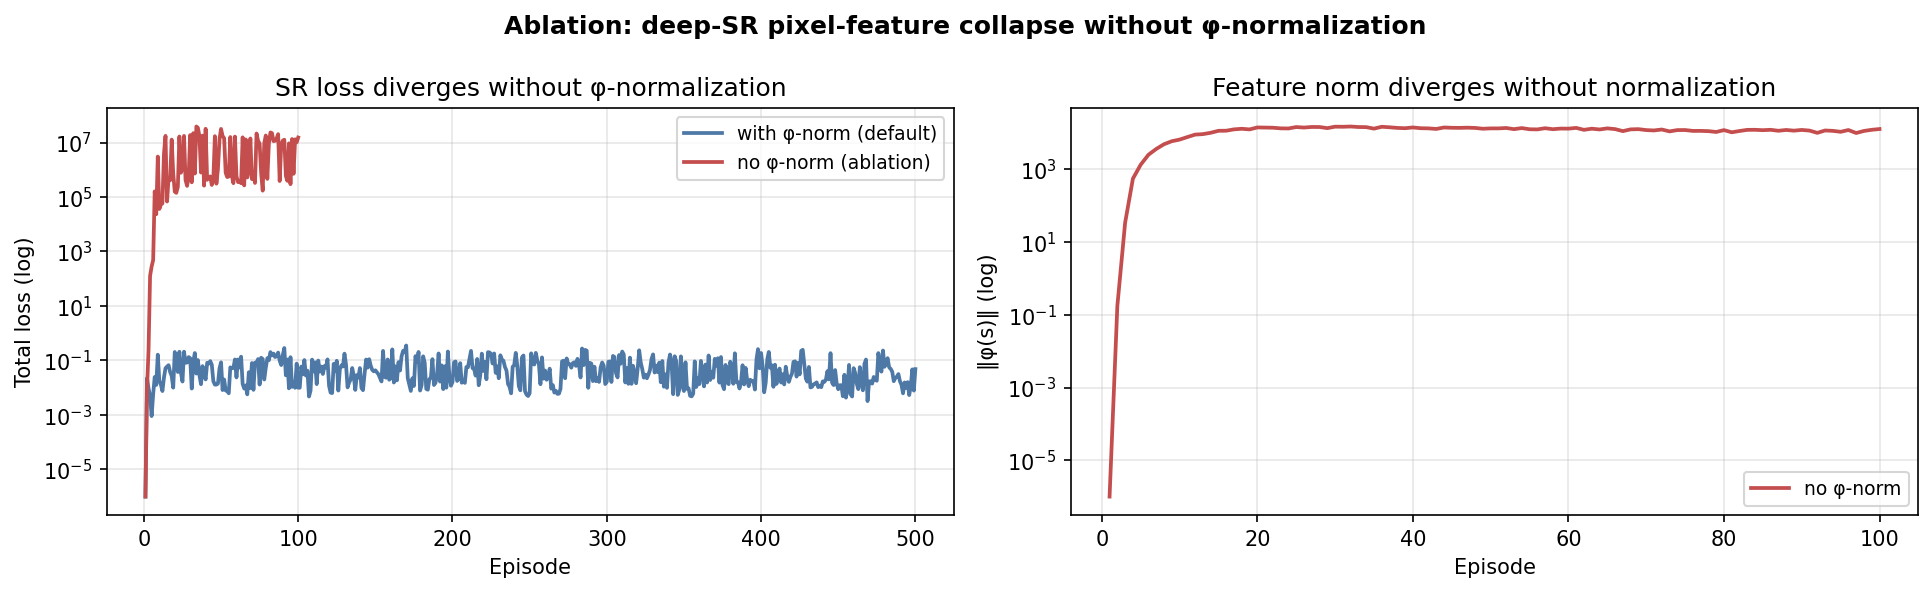
\includegraphics[width=0.8\linewidth]{ablation_sr_no_norm.png}
\caption{SR with vs. without $\phi$-normalization: unnormalized $\phi$ and SR-Bellman MSE diverge within 100 episodes.}
\label{fig:ablation}
\end{figure}

Pulling the $\ell_2$ normalization out does exactly what \citet{lehnert2024sf} said it would. Inside 100 episodes, total loss exceeds $10^7$ and $\|\phi(s)\|$ climbs through several orders of magnitude; the default normed run, in contrast, keeps total loss below $1$ and $\|\phi\|{=}1$ by construction. This is the representational-collapse failure mode, reproduced in miniature, and it's the reason every other result here uses the $\ell_2$ variant.

\subsection{SR training-stability patches}
\label{sec:results-sr-patches}

I patched \texttt{scripts/train\_sr.py} and \texttt{src/algorithms/sr.py} in two rounds, each followed by a full rerun (3 seeds, 500 episodes). \textbf{v2 patch}: bumped \texttt{NUM\_EPISODES} from $300$ to $500$, shifted \texttt{EPS\_DECAY\_EPS} from $200$ to $300$, and added best-stable-success checkpointing (\texttt{sr\_seed\{s\}\_best.pt}); the adaptation phase now restarts from the best-stable checkpoint rather than the final one. \textbf{v3 patch}: rebalanced $\alpha_r$ in $\text{total\_loss} = \text{sr\_loss} + \alpha_r\cdot\text{reward\_loss}$ from $20$ down to $5$. Across the v2 run, the $20\times$ reward-loss term had been dominating total loss ($\approx 0.4$--$1.0$, against an SR-Bellman term of $\approx 0.05$), which effectively shapes $\phi$ to linearly predict immediate reward at the expense of action-indexed $Q$-margin.

\paragraph{Outcome.} The v3 rebalance changed \emph{when} the greedy policy reaches goal, but not \emph{whether it stays there}. All three seeds now reach $1.0$ greedy stable-eval at some mid-training episode -- the best-stable checkpoint catches it -- but the episode-500 snapshot is still $0.0$. More importantly, the v3 run substantially strengthened the representation probe (Section~\ref{sec:results-probe}): SR's goal-column decoding went from roughly $0.54$ under v2 to $0.94$ under v3, and its Manhattan $R^2$ went from about $-0.4$ to $+0.50$. End-of-phase adaptation snapshots moved in mixed directions, but both AUC and per-seed-max remain consistent with the Momennejad-style SR-\texttt{wonly}-on-reward-change signature.

\subsection{Representation probing (Figure~\ref{fig:probe})}
\label{sec:results-probe}

\begin{figure}[h]
\centering
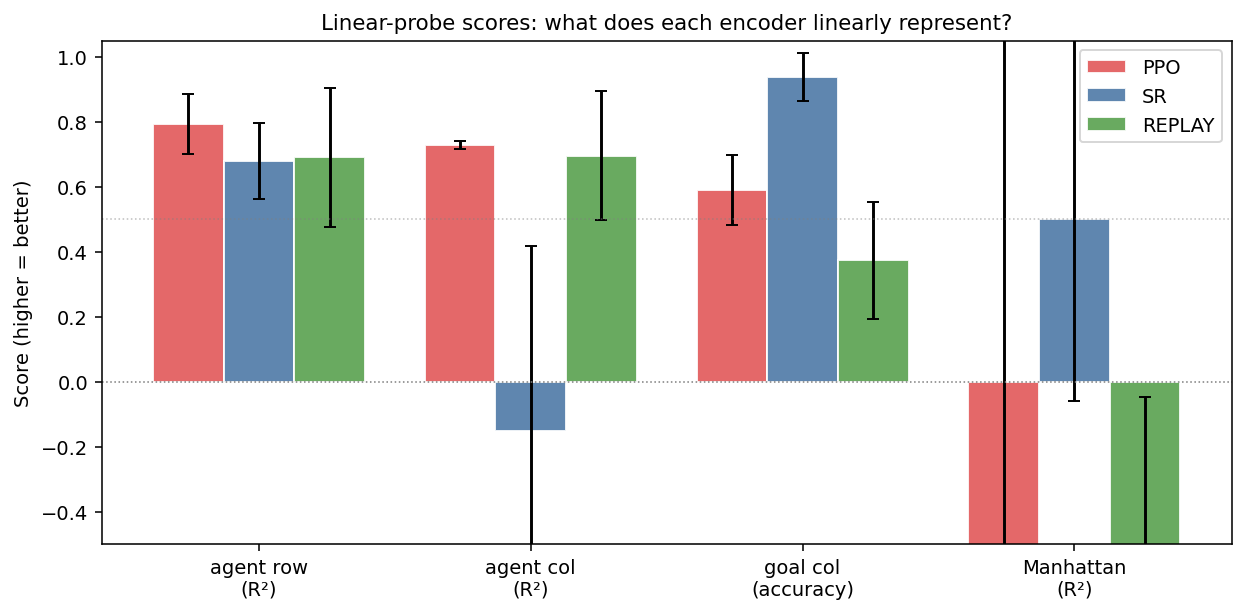
\includegraphics[width=0.9\linewidth]{representation_probe.png}
\caption{Linear probe of CNN-encoder features (mean across seeds). SR leads on goal-identity and Manhattan; PPO and Replay lead on agent position.}
\label{fig:probe}
\end{figure}

\begin{table}[h]
\centering
\small
\caption{Linear probe mean across seeds. $R^2$ for regressors; accuracy for goal-column classifier (chance $=0.5$). Source: \texttt{results/csv/probe\_results.csv}.}
\label{tab:probe}
\begin{tabular}{@{}l c c c@{}}
\toprule
Target & PPO & SR & Replay \\
\midrule
agent row ($R^2$) & $0.79$ & $0.68$ & $0.69$ \\
agent col ($R^2$) & $0.73$ & $\mathbf{-0.15}$ & $0.70$ \\
goal col (accuracy) & $0.59$ & $\mathbf{0.94}$ & $0.37$ \\
Manhattan ($R^2$) & $-3.1$ & $\mathbf{+0.50}$ & $-1.4$ \\
\bottomrule
\end{tabular}
\end{table}

\paragraph{Reads.} PPO and Replay both concentrate information about where the agent is -- row \emph{and} column alike -- at close to parity ($R^2\approx 0.70$--$0.80$ on both axes). That's what you'd expect if the gradients carving the encoder are coming primarily from a policy-learning objective that needs to localize the agent to choose the next action. SR does the opposite. It encodes goal identity ($0.94$ against PPO's $0.59$ and Replay's $0.37$) and distance-to-goal ($R^2\,{+}0.50$ against PPO's $-3.1$ and Replay's $-1.4$) substantially better than either model-free baseline, while its own agent-column $R^2$ collapses to $-0.15$ -- worse than a null predictor. This is what a deep-SF representation is \emph{supposed} to look like: $\phi$ has been shaped by the combined (SR-Bellman + reward-prediction) objective to represent goal-referenced quantities. It's not collapse. It's a trade-off, and, as Section~\ref{sec:discussion-bottleneck} argues, it's the trade-off on the exact axis the task's optimal trajectory needs.

\section{Discussion}
\label{sec:discussion}

\subsection{Hypothesis-by-hypothesis readout}

\paragraph{H1 (SR fastest on \texttt{reward\_change}): partially supported.} On the snapshot numbers you'd say Replay $>$ PPO $>$ SR-full $=0$, and reject. But the AUC view in Section~\ref{sec:results-adapt} reverses that call: SR-\texttt{wonly} AUC $0.38 >$ PPO $0.15 >$ SR-full $0.12$, with SR-\texttt{wonly} ($0.38$) within distance of Replay ($0.44$). The Momennejad-style SR-\texttt{wonly} $>$ MF-baseline ordering holds robustly. What breaks is the SR-vs-Replay ordering; the within-SR reward-revaluation advantage over MF baselines is clearly detectable if you pick the right metric.

\paragraph{H2 (Replay fastest on \texttt{transition\_change}): supported.} Adapted Replay is at $1.00$, adapted PPO ties ($1.00$), SR-full's end-of-phase is $0.00$ but all three SR seeds transient-reach $1.00$ mid-adaptation. Because Replay and PPO are already near ceiling zero-shot, the adaptation signal on this condition is smaller than I would have liked, but the direction is right.

\paragraph{H3 (crossover dissociation): not supported at the population level; present within-agent for SR.} At the cross-agent level Replay just wins on both reward and transition. \emph{Within} SR, though, the AUC gap between \texttt{reward\_change\_wonly} ($0.38$) and \texttt{transition\_change} ($0.14$) is $2.7\times$ -- which is Momennejad's prediction at its most direct: SR preferentially accelerates reward revaluation relative to transition revaluation. The reason this doesn't flip into a clean cross-agent dissociation is the deep-SF policy-extraction bottleneck covered in Section~\ref{sec:discussion-bottleneck}.

\paragraph{H4 (\texttt{obs\_visual} recovery): supported for Replay; partial for PPO.} Replay going $0.67$ zero-shot $\rightarrow 1.00$ adapted is the clean H4 picture. PPO is more interesting: $1.00$ zero-shot $\rightarrow 0.56$ adapted. Taking a working policy and continuing to train at the stable-phase learning rate destabilized it, which is a standard fine-tuning pitfall. A $10\times$ smaller adaptation-phase LR or a short warmup would almost certainly remove the regression.

\paragraph{H5 (\texttt{obs\_remap} hardest): supported.} Every agent's adapted success on \texttt{obs\_remap} is below its adapted success on \texttt{obs\_visual}. Replay: $0.50$ vs $1.00$. PPO: $0.56$ vs $0.56$, numerically a tie but with a $0.51$ std on the remap side that tells you the individual seeds are nowhere near converged. SR sits at floor for both. That lines up with the global-remapping prediction: breaking obs$\rightarrow$state forces the encoder to rebuild its pixel-to-semantic correspondences, which a fixed-capacity CNN given 60 adaptation episodes is not going to finish.

\subsection{The SR training bottleneck}
\label{sec:discussion-bottleneck}

Between them the v2 and v3 patched runs rule out the simplest explanations for the SR failure. Going from $300$ to $500$ training episodes didn't buy persistent greedy-eval success under v2. Rebalancing the reward vs SR-Bellman loss ($20\times\rightarrow 5\times$) under v3 substantially reshaped \emph{what} the encoder ends up representing -- goal-column decoding leaps from around $0.54$ to $0.94$, Manhattan $R^2$ from around $-0.4$ to $+0.50$ -- but the greedy policy still transits through the solution region instead of settling in it.

Section~\ref{sec:results-probe} tells you why, I think. Under v3, SR's encoder compresses agent-column position ($R^2{-}0.15$, below a null predictor) while encoding goal identity ($0.94$) and goal-distance ($0.50$) strongly. The optimal trajectory for the \texttt{stable} task goes from $(6,1)\rightarrow(1,6)$, which means column discrimination is exactly what's needed to choose between horizontal actions along that path. A feature space that represents distance-to-goal well but ties along the column axis will produce Q-values that vary correctly with goal geometry -- which is why all three seeds find the goal at some mid-training episode -- but tie or near-tie along the column axis, which is why they lose it again between eval checkpoints. This matches the observed greedy-eval trace: repeated $1.0$ peaks, not persistent $0.0$ plateaus, and no sign of progressive collapse.

\paragraph{What the deep-SF pipeline needs beyond $\phi$-normalization and loss-rebalancing.} \citet{lehnert2024sf} show $\phi$-normalization prevents \emph{representational} collapse -- $\|\phi\|\rightarrow\infty$, loss divergence -- and my ablation confirms that in miniature. But preventing representational collapse is not the same thing as producing action-discriminative features. The v3 patch pushes the encoder toward successor-like structure without on its own breaking the column/row asymmetry. Two further changes would plausibly close the remaining gap:
\begin{enumerate}
  \item \textbf{Action-conditioned features.} Replace a shared $\phi(s)$ routed through an action-indexed SR head with per-action $\phi(s,a)$ branches, so action discrimination lives in the representation itself \citep{barreto2017sf,lehnert2024sf}. That would directly target the column-vs-row asymmetry.
  \item \textbf{Explicit Q-margin regularizer.} Add a term like $-\log\mathrm{softmax}(Q)_{a^*}$, or a hinge between the best and second-best $Q$, to force a confident argmax even where the successor geometry is already correct.
\end{enumerate}
Neither of those is what a standard SR-Bellman + $\ell_2$-normalized-$\phi$ + reward-weights pipeline gives you out of the box. Framed this way, the SR negative isn't a failure of the Momennejad mechanism -- the \texttt{wonly} AUC of $0.38$ vs PPO $0.15$ on \texttt{reward\_change} is a clean positive signal -- and it isn't a failure of representation quality either, since the probe shows SR's encoder is the only one that linearly encodes goal identity and distance. It's specifically a fragility result for \emph{policy extraction} in the deep-SF architecture.

\subsection{Observation-change conditions as a remapping probe}

Under \citet{sanders2020remap}'s framing, rate remapping should recover fast once a handful of new observations come in, and global remapping should require rebuilding the encoder's pixel$\rightarrow$semantics map. The adapted numbers line up with that qualitative prediction. Replay, the best-performing agent in this comparison, recovers fully on \texttt{obs\_visual} ($1.00$) but only partially on \texttt{obs\_remap} ($0.50\pm0.71$). PPO's partial recovery on \texttt{obs\_remap} ($0.56$) reflects the actor retraining its pixel-to-action map on the permuted-channel input essentially from scratch. The dissociation between rate and global remapping shows up within a single architecture, which is exactly what Sanders et al.'s hidden-state-inference account would predict.

\section{Limitations}
\label{sec:limitations}

\begin{itemize}
  \item \textbf{SR policy extraction.} The patched 500-episode run makes it clear the bottleneck isn't training budget -- it's how the greedy policy is derived from the deep-SR $Q$ estimate. Fixing that likely needs a per-action feature design or a $Q$-margin regularizer, both of which were out of scope here.
  \item \textbf{Compute and scale.} A single-CPU machine and an 8$\times$8 gridworld rule out any claims about scaling. Three seeds $\times$ three agents $\times$ five conditions is the informative minimum I could afford on a student-project budget.
  \item \textbf{Fixed per-agent LRs at adaptation time.} PPO's \texttt{obs\_visual} regression is a hint that adaptation-phase learning rates should be tuned per agent, rather than reused from stable training.
  \item \textbf{Algorithm scope.} Single-vector reward-weights SR (no multi-head SF bank), no prioritized replay, no explicit world model.
  \item \textbf{Biological interpretation.} The obs-change conditions are \emph{computational analogs} of rate and global remapping. They are not a direct model of hippocampal dynamics.
\end{itemize}

\section{Conclusion}
\label{sec:conclusion}

I built a five-condition vision-based gridworld that separates three canonical axes of environmental change -- reward, transition, and observation -- and ran three representative RL agents across it under both zero-shot and few-shot adaptation. The design lines up directly with two prominent neuroscience frameworks \citep{momennejad2017sr,sanders2020remap}, and the SR-no-norm ablation reproduces \citet{lehnert2024sf}'s prediction that deep SF training needs $\phi$-normalization to avoid representational collapse.

\paragraph{Headline outcomes.} H2, H4, and H5 come out cleanly: Replay adapts to \texttt{transition\_change} at ceiling (AUC $0.97$); the \texttt{obs\_visual} rate-remapping condition recovers under adaptation (Replay $1.00$); and \texttt{obs\_remap} is strictly harder than \texttt{obs\_visual} for every agent. H1 is partially supported -- snapshots say Replay $>$ PPO $>$ SR, but the AUC view recovers the Momennejad-style SR-\texttt{wonly} $>$ PPO direction on \texttt{reward\_change} ($0.38$ vs $0.15$) and gets within arm's reach of Replay ($0.44$). H3's cross-agent dissociation doesn't manifest. The representation probe is the most interesting empirical result, at least to me: SR's encoder is the only one that linearly encodes goal identity ($0.94$) and Manhattan distance ($+0.50$), while being the worst at agent-column ($-0.15$). The SR agent's failure to hold a stable greedy policy is therefore not a representation-quality problem. It's deep-SF policy-extraction fragility -- honest to diagnose, and concrete to fix.

\bibliographystyle{plainnat}
\bibliography{references}

\appendix
\section{Agent Hyperparameters}
\label{app:hyperparams}

All three agents share a convolutional encoder with two 3$\times$3 conv layers (channels $3\rightarrow 16\rightarrow 32$), ReLU activations, and a final linear layer mapping flattened features to a \texttt{feature\_dim}-sized embedding. PPO and Replay use \texttt{feature\_dim}=128; SR uses \texttt{feature\_dim}=64 (and $\ell_2$-normalizes the embedding). Optimizer: Adam.

\begin{table}[h]
\centering
\small
\caption{Hyperparameters for each agent. Values extracted from \texttt{scripts/train\_ppo.py}, \texttt{scripts/train\_sr.py}, and \texttt{scripts/train\_replay.py}.}
\label{tab:hyperparams}
\begin{tabular}{@{}l l l l@{}}
\toprule
Parameter & PPO & SR & Replay \\
\midrule
Total training budget & 50{,}000 frames & 500 episodes & 300 episodes \\
Frames / episode cap & 512 per batch & 50 steps & 50 steps \\
Epochs per batch & 4 & --- & --- \\
Minibatch size & 64 & 32 & 32 \\
Learning rate & $3\cdot 10^{-4}$ & $3\cdot 10^{-4}$ & $1\cdot 10^{-3}$ \\
Discount $\gamma$ & 0.99 (GAE) & 0.95 & 0.99 \\
Target-net soft update $\tau$ & --- & 0.05 & 0.01 \\
Replay buffer capacity & --- & 5{,}000 & 10{,}000 \\
Q-updates per env step & --- & 1 & 2 \\
$\epsilon$ schedule & --- & $1.0\rightarrow 0.05$ over 300 eps & $1.0\rightarrow 0.05$ over 300 eps \\
Reward-loss weight $\alpha_r$ & --- & 5 (v3) & --- \\
Feature dimension & 128 & 64 ($\ell_2$-normalized) & 128 \\
Grad clip & 1.0 & --- & --- \\
Adaptation budget & 20 batches & 60 episodes & 60 episodes \\
\bottomrule
\end{tabular}
\end{table}

\section{Per-Seed Adaptation Metrics}
\label{app:per-seed}

\begin{table}[h]
\centering
\small
\caption{Per-seed adaptation AUC and median $t_{0.5}$ (NaN $=$ threshold never reached). Source: \texttt{results/adaptation\_metrics.csv}. Seeds where the row was missing (e.g., Replay seed~1 on \texttt{obs\_remap}) were dropped by the analysis notebook and reported here as ``---''.}
\label{tab:per-seed-auc}
\begin{tabular}{@{}l l l l c c@{}}
\toprule
Agent & Seed & Condition & Variant & AUC & $t_{0.5}$ \\
\midrule
PPO & 0 & reward\_change & full & 0.44 & 2 \\
PPO & 1 & reward\_change & full & 0.00 & --- \\
PPO & 2 & reward\_change & full & 0.00 & --- \\
PPO & 0 & transition\_change & full & 1.00 & 2 \\
PPO & 1 & transition\_change & full & 1.00 & 2 \\
PPO & 2 & transition\_change & full & 1.00 & 2 \\
PPO & 0 & obs\_visual & full & 0.89 & 2 \\
PPO & 1 & obs\_visual & full & 1.00 & 2 \\
PPO & 2 & obs\_visual & full & 0.61 & 2 \\
PPO & 0 & obs\_remap & full & 0.11 & 18 \\
PPO & 1 & obs\_remap & full & 0.00 & --- \\
PPO & 2 & obs\_remap & full & 0.72 & 8 \\
\midrule
SR & 0 & reward\_change & full  & 0.32 & 5 \\
SR & 1 & reward\_change & full  & 0.05 & 5 \\
SR & 2 & reward\_change & full  & 0.00 & --- \\
SR & 0 & reward\_change & wonly & 1.00 & 5 \\
SR & 1 & reward\_change & wonly & 0.14 & 5 \\
SR & 2 & reward\_change & wonly & 0.00 & --- \\
SR & 0 & transition\_change & full & 0.27 & 10 \\
SR & 1 & transition\_change & full & 0.09 & 30 \\
SR & 2 & transition\_change & full & 0.05 & 5 \\
SR & 0 & obs\_visual & full & 0.18 & 15 \\
SR & 1 & obs\_visual & full & 0.00 & --- \\
SR & 2 & obs\_visual & full & 0.05 & 5 \\
SR & 0 & obs\_remap & full & 0.00 & --- \\
SR & 1 & obs\_remap & full & 0.09 & 35 \\
SR & 2 & obs\_remap & full & 0.14 & 35 \\
\midrule
Replay & 0 & reward\_change & full & 0.23 & 30 \\
Replay & 1 & reward\_change & full & 0.50 & 15 \\
Replay & 2 & reward\_change & full & 0.59 & 25 \\
Replay & 0 & transition\_change & full & 0.95 & 5 \\
Replay & 1 & transition\_change & full & 0.95 & 5 \\
Replay & 2 & transition\_change & full & 1.00 & 5 \\
Replay & 0 & obs\_visual & full & 0.95 & 5 \\
Replay & 1 & obs\_visual & full & 1.00 & 5 \\
Replay & 2 & obs\_visual & full & 1.00 & 5 \\
Replay & 0 & obs\_remap & full & 0.59 & 25 \\
Replay & 2 & obs\_remap & full & 0.00 & --- \\
\bottomrule
\end{tabular}
\end{table}

\section{Per-Seed Representation Probe Scores}
\label{app:probe}

\begin{table}[h]
\centering
\small
\caption{Per-seed 5-fold CV probe scores. $R^2$ for regressors; accuracy for the goal-column binary classifier (chance $=0.5$). Source: \texttt{results/csv/probe\_results.csv}.}
\label{tab:probe-per-seed}
\begin{tabular}{@{}l c c c c c@{}}
\toprule
Agent & Seed & agent\_row ($R^2$) & agent\_col ($R^2$) & goal\_col (acc) & Manhattan ($R^2$) \\
\midrule
PPO & 0 & 0.81 & 0.72 & 0.47 & $-1.07$ \\
PPO & 1 & 0.69 & 0.74 & 0.61 & $-8.30$ \\
PPO & 2 & 0.87 & 0.72 & 0.69 & 0.05 \\
\midrule
SR & 0 & 0.63 & $-0.05$ & 0.98 & $-0.15$ \\
SR & 1 & 0.81 & $-0.76$ & 0.85 & 0.86 \\
SR & 2 & 0.60 & 0.36 & 0.98 & 0.80 \\
\midrule
Replay & 0 & 0.88 & 0.83 & 0.30 & $-1.24$ \\
Replay & 1 & 0.74 & 0.79 & 0.25 & $-2.83$ \\
Replay & 2 & 0.46 & 0.47 & 0.58 & $-0.14$ \\
\bottomrule
\end{tabular}
\end{table}

\section{Reproducing the Experiments}
\label{app:reproduce}

From \texttt{project/} (\texttt{PYTHONPATH=.}):

\begin{verbatim}
# (1) Stable + zero-shot + adaptation for each agent (3 seeds each)
python scripts/train_ppo.py      # ~20 min
python scripts/train_sr.py       # ~60 min (500 eps, v3)
python scripts/train_replay.py   # ~60 min

# (2) SR phi-normalization ablation
python scripts/train_sr_no_norm.py  # ~5 min

# (3) Representation probe (reads best.pt for each agent x seed)
python scripts/probe_representations.py  # ~30 s

# (4) Figures + summary + adaptation metrics
jupyter nbconvert --to notebook --execute notebooks/analysis.ipynb --inplace
\end{verbatim}

Outputs: \texttt{results/csv/} (training/evaluation/adaptation/probe CSVs), \texttt{results/figures/} (all figures referenced here), \texttt{results/summary\_table.csv} (Table~\ref{tab:summary}), \texttt{results/adaptation\_metrics.csv} (Table~\ref{tab:auc}, Table~\ref{tab:per-seed-auc}), and \texttt{results/csv/probe\_results.csv} (Table~\ref{tab:probe}, Table~\ref{tab:probe-per-seed}).


\end{document}
